%-----------------------------------------------------------------------------%
\chapter{\babEmpat}
%-----------------------------------------------------------------------------%
Bab ini akan membahas hasil penelitian yang telah dilakukan dan analisis terhadap
hasil penelitian tersebut. 

%-----------------------------------------------------------------------------%
\section{Hasil Penelitian}
%-----------------------------------------------------------------------------%
\hspace{0.5cm}Berdasarkan kerangka penelitian yang telah dijelaskan pada bab sebelumnya, terdapat 10 skenario percobaan dimana masing - masing 5 skenario pada aplikasi Autodock dan 5 skenario pada aplikasi Autodock Vina. Secara garis besar, skenario tersebut adalah menjalankan aplikasi yang telah terpasang pada \textit{container} Docker yang telah dibuat. Untuk setiap skenario jumlah data pada masing - masing \textit{container} akan dibagi berdasarkan total data (1406 data \textit{receptor}) dibagi dengan jumlah \textit{container} yang terbentuk. Setelah data terbagi, masing - masing \textit{container} akan menjalankan aplikasi (Autodock ataupun Autodock Vina) dan waktu akan dicatat dari awal eksekusi data pertama hingga waktu akhir ketika aplikasi selesai mengeksekusi data terakhir.

Berikut merupakan data yang diperoleh dari 5 skenario aplikasi Autodock Vina

\begin{table}[h]
	\centering
	\begin{tabular}{|c|l|l|l|}
		\hline
		\multirow{2}{*}{Jumlah \textit{container}} & \multicolumn{3}{c|}{Waktu eksekusi (menit)} \\ \cline{2-4} 
		& \multicolumn{1}{c|}{tercepat} & \multicolumn{1}{c|}{terlama} & \multicolumn{1}{c|}{Rata-rata} \\ \hline
		50 & 625 & 1359 & 968 \\ \hline
		100 & 407 & 1434 & 891 \\ \hline
		150 & 247 & 2615 & 745 \\ \hline
		200 & 129 & 1496 & 705 \\ \hline
		250 & 193 & 1431 & 720 \\ \hline
	\end{tabular}
		\caption{Hasil skenario eksperimen pada aplikasi Autodock Vina}
		\label{my-label}
\end{table}

Untuk masing - masing data waktu eksekusi tersebut dapat disajikan menjadi tabel grafik. Tabel yang disajikan berupa waktu eksekusi tercepat, terlama dan rata - rata eksekusi setiap \textit{container} untuk setiap skenario.

\begin{figure}
	\centering
	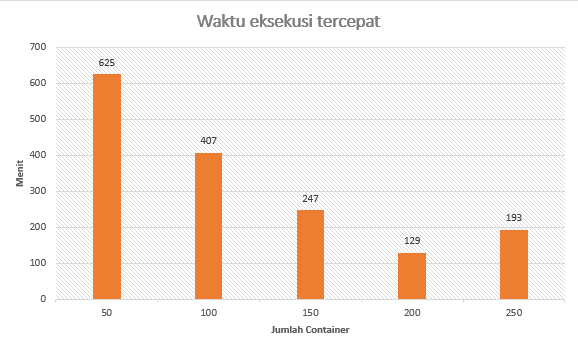
\includegraphics{tercepat_vina.PNG}
	\caption{Waktu eksekusi tercepat untuk masing - masing skenario Autodock Vina}
\end{figure}
 
\begin{figure}
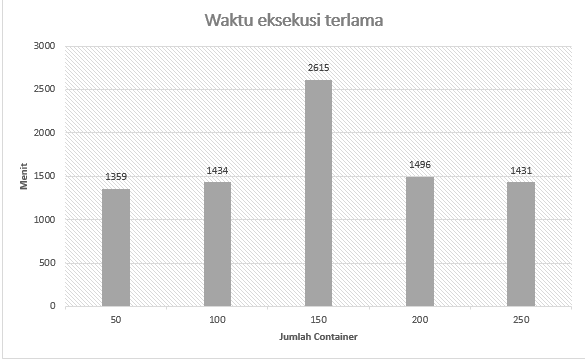
\includegraphics{terlama_vina.PNG}
\caption{Waktu eksekusi terlama untuk masing - masing skenario Autodock Vina}
\end{figure}

\begin{figure}
	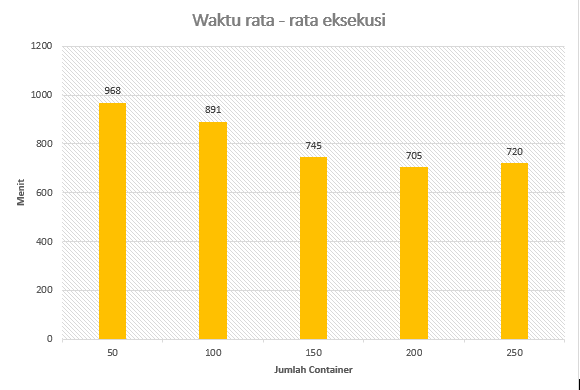
\includegraphics{ratarata_vina.PNG}
	\caption{Grafik dari rata - rata waktu eksekusi masing - masing skenario Autodock Vina}
\end{figure}

Berikut merupakan data yang diperoleh dari 5 skenario aplikasi Autodock 
\begin{table}
	\centering
	\begin{tabular}{|c|l|l|l|}
		\hline
		\multirow{2}{*}{Jumlah \textit{container}} & \multicolumn{3}{c|}{Waktu eksekusi (menit)} \\ \cline{2-4} 
		& \multicolumn{1}{c|}{tercepat} & \multicolumn{1}{c|}{terlama} & \multicolumn{1}{c|}{Rata-rata} \\ \hline
		50 & 1044 & 1344 & 1255 \\ \hline
		100 & 835 & 1386 & 1259 \\ \hline
		150 & 710 & 1405 & 1216 \\ \hline
		200 & 482 & 1276 & 1007 \\ \hline
		250 & 358 & 1071 & 811 \\ \hline
	\end{tabular}
	\caption{Hasil skenario pada eksperimen Autodock}
	\label{my-label}
\end{table}

Untuk masing - masing data waktu eksekusi tersebut dapat disajikan menjadi tabel grafik :

\begin{figure}
	\centering
	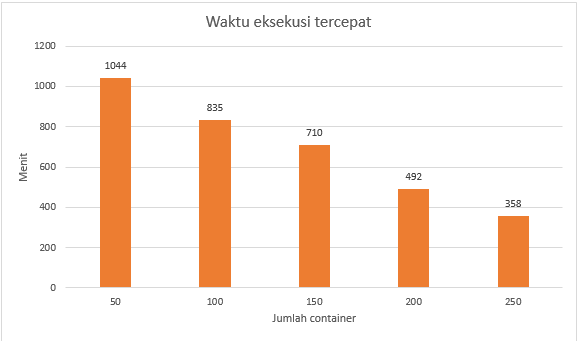
\includegraphics{tercepat_dock.PNG}
	\caption{Waktu eksekusi tercepat untuk masing - masing skenario Autodock}
\end{figure}

\begin{figure}
	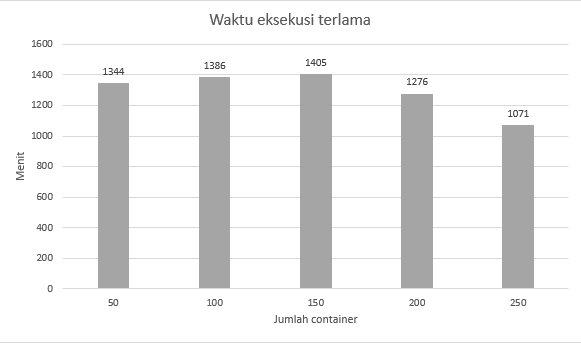
\includegraphics{terlama_dock.PNG}
	\caption{Waktu eksekusi terlama untuk masing - masing skenario Autodock}
\end{figure}

\begin{figure}
	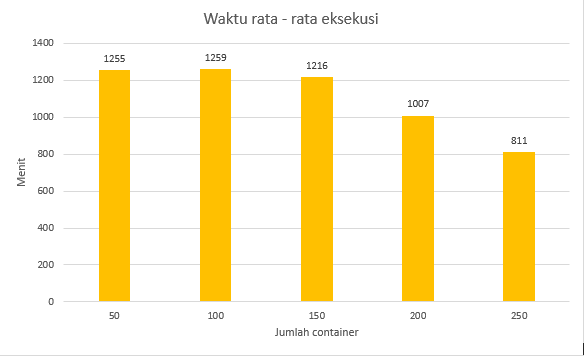
\includegraphics{ratarata_dock.PNG}
	\caption{Grafik rata - rata waktu eksekusi masing - masing skenario Autodock}
\end{figure}

%-----------------------------------------------------------------------------%
\section{Analisis}
%-----------------------------------------------------------------------------%
\hspace{0.5cm}Pada situs resmi Autodock telah ditampilkan perbandingan performa antara Autodock dan Autodock Vina \cite{comparison_dockvina} seperti berikut :
 
\begin{figure}
	\centering
	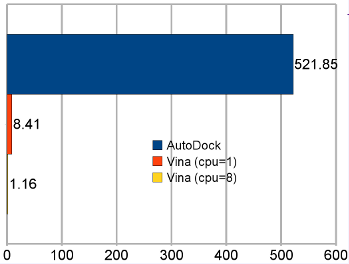
\includegraphics{comparison_dockvina.PNG}
	\caption{Perbandingan waktu \textit{running} pada situs resmi Autodock \cite{autodockvina}}
\end{figure}

Eksekusi pada Autodock Vina jauh lebih cepat dibandingkan dengan Autodock, hal ini dikarenakan pada aplikasi Autodock Vina memanfaatkan \textit{multithreading} sehingga dapat mengoptimalkan kinerja dari banyak CPU \cite{autodockvina}. Gambar 4.7 diatas memberikan gambaran awal bahwa dalam skenario penelitian yang dilakukan, Autodock Vina akan memberikan waktu eksekusi yang lebih cepat dibandingkan dengan Autodock. Untuk setiap rata - rata waktu eksekusi pada skenario Autodock Vina dibandingkan dengan rata - rata waktu eksekusi pada skenario Autodock memberikan hasil yang sama dengan grafik yang diberikan pada situs resmi Autodock.

Pada tabel waktu rata - rata eksekusi untuk aplikasi Autodock dan Autodock Vina dapat dilihat bahwa grafik dari setiap skenario memberikan \textit{trend} menurun. Dengan begitu dapat dilihat bahwa jumlah \textit{container} dan jumlah data menjadi faktor yang mempengaruhi waktu proses tersebut. Dapat disimpulkan bahwa, semakin banyak \textit{container} yang dibentuk maka semakin sedikit data yang digunakan pada aplikasi Autodock maupun Autodock Vina pada masing - masing \textit{container}. Semakin banyak \textit{container} juga memperbanyak eksekusi aplikasi yang dilakukan secara paralel. Pada gambar  grafik 4.3 dan 4.6 diatas terlihat \textit{trend} semakin banyak \textit{container} maka waktu eksekusi akan semakin sedikit. Namun dapat dilihat juga pada gambar tabel 4.3, \textit{container} 200 menghasilkan waktu eksekusi yang lebih kecil dibandingkan dengan \textit{container} 250. Penulis memperkirakan bahwa kompleksitas molekul juga mengambil andil dalam lamanya waktu yang dibutuhkan oleh aplikasi Autodock maupun Autodock Vina. Untuk dapat memastikan bahwa jumlah \textit{container} mempengaruhi, penulis mencoba untuk menghitung waktu eksekusi aplikasi Autodock dan Autodock Vina dalam memproses 1406 data receptor.

\begin{table}
	\centering
	\begin{tabular}{|c|c|c|}
		\hline
		\multicolumn{3}{|c|}{Waktu eksekusi (menit)} \\ \hline
		Jumlah Container & Autodock & Autodock Vina \\ \hline
		1 & 4797 & 1459 \\ \hline
	\end{tabular}
	\caption{Waktu eksekusi Autodock dan Autodock Vina saat 1 \textit{container}}
	\label{my-label}
\end{table}

Dapat dilihat pada tabel 4.3 bahwa waktu yang dibutuhkan dalam menjalankan skenario percobaan dengan hanya menggunakan 1 buah \textit{container} memakan waktu yang lebih lama dibandingkan dengan banyak \textit{container} pada skenario penelitian.

Dari skenario yang telah dilakukan, penulis juga mengamati kinerja CPU dan memori yang digunakan oleh Docker. Berdasarkan penjelasan Marek Goldmann \cite{Marek Goldmann} , setiap \textit{container} yang dibentuk akan membagi sama rata \textit{resource} CPU. Pembagian tersebut hanyalah \textit{relative weight}, dimana setiap \textit{container} dapat menggunakan \textit{shared} CPU, bukan kecepatan kasar CPU yang digunakan oleh \textit{container}. Container yang terbentuk awalnya akan memiliki 1024 \textit{shared} CPU dari CPU fisik, dan akan terbagi sama rata selama \textit{container} baru akan terbentuk. Hasil dari penelitian ini baik menjalankan aplikasi Autodock maupun Autodock Vina dapat dilihat sebagai berikut :
\begin{table}
	\centering
	\begin{tabular}{|c|c|c|}
		\hline
		\multicolumn{3}{|c|}{\textit{Relative weight} CPU (\%)} \\ \hline
		Jumlah \textit{container} & Autodock Vina & Autodock \\ \hline
		50 & 15,9 - 16,9 & 15,6 -19,6 \\ \hline
		100 & 7,9 - 12,3 & 8 - 8,6 \\ \hline
		150 & 5 - 5,6 & 6-7,6 \\ \hline
		200 & 3,3 - 3,9 & 4,6 - 5 \\ \hline
		250 & 0,7 - 3 & 3,6 - 4 \\ \hline
	\end{tabular}
	\caption{Persentasi \textit{relative weight} pemanfaatan CPU}
	\label{my-label}
\end{table}

Walaupun dari tabel diatas tidak seperti perhitungan yang dikatakan oleh Marek Goldmann, angka - angka tersebut tetap mendekati pembagian secara merata. Penelitian yang dilakukan menggunakan \textit{desktop} CPU dengan  prosesor Intel i-7 , dimana prosesor secara fisik memiliki 4 core namun dengan adanya \textit{Hyper Threading}, terdapat logical core untuk masing - masing core sehingga terbaca menjadi 8 core (800 \%). Dalam kenyataannya, nilai \textit{relative weight} dapat berubah mengikuti besarnya \textit{task} yang dikerjakan oleh \textit{container} tersebut dan nilai \textit{relative weight} \textit{container} lain. Nilai \textit{relative wieght container} dalam keadaan \textit{idle} dapat terbagi sama rata untuk \textit{container} lain yang masih mengerjakan \textit{task} (menyesuaikan dengan \textit{task} dalam \textit{container}). Dalam hal pembagian memori, setiap \textit{container} dapat menggunakan memori pada \textit{host} hingga kapasitas maksimum memori pada \textit{host}. Pada eksperimen yang dijalankan, terlihat bahwa untuk aplikasi Autodock Vina maupun Autodock yang dijalankan hanya menggunakan 0,1 \% - 0,9 \% dari memori pada komputer \textit{host}

Dalam penelitian ini penulis juga membandingkan performa yang diberikan oleh Docker dengan penelitian yang telah dilakukan oleh Muhammad H. Hilman \cite{cloud_pak hilman}. Beliau menggunakan aplikasi Autodock Vina dalam \textit{virtual screening}. Perbandingan dilakukan dengan mencari waktu untuk memproses 1 buah molekul. Waktu ini didapat dengan membagi waktu yang dihasilkan dari awal eksekusi aplikasi Autodock maupun Autodock Vina pada \textit{container} hingga aplikasi selesai bekerja dengan jumlah data yang digunakan dalam eksperimen penelitian, yaitu 1406 buah data. Berikut merupakan gambar tabel waktu yang dibutuhkan dalam memproses 1 molekul yang dapat dikerjakan dalam \textit{virtual cluster} dalam Amazon EC2 :
\begin{table}
	\centering
	\begin{tabular}{|c|c|c|c|}
		\hline
		Parameter & SCluster & LCluster & XLCluster \\ \hline
		Memory & 1,7 GB & 7,5GB & 15 GB \\ \hline
		Compute Unit / Processors & 1,2 GHz X 1 & 1,2 GHz X 4 & 1,2 GHz X 8 \\ \hline
		Platform & 32-bit & 64-bit & 64-bit \\ \hline
		Harga/jam & \$0,085 & \$0,34 & \$0,68 \\ \hline
	\end{tabular}
\caption{Spesifikasi harga dan \textit{resource cloud computing} yang disediakan oleh Amazon EC2 \cite{cloud_pak hilman}}
	\label{my-label}
\end{table}
Berdasarkan penelitian yang dilakukan sebelumnya, masing - masing \textit{cluster} terdiri dari 4 node. \textit{Hardware} komputasi tidak sama untuk masing - masing \textit{cluster}, Amazon memberikan gambaran besarnya \textit{clock speed} dan berapa jumlah \textit{processor}.  
\begin{table}
	\centering
	\begin{tabular}{|l|l|l|l|}
		\hline
		Parameter & SCluster & LCluster & XLCluster \\ \hline
		Total ExecTime(s) & 375.624 & 108.179 & 48.421 \\ \hline
	\end{tabular}
	\caption{Hasil pengukuran \textit{virtual screening} \cite{cloud_pak hilman}}
	\label{my-label}
\end{table}
Tabel diatas merupakan hasil waktu yang diperoleh dalam menjalankan Autodock Vina pada jasa \textit{cloud computing} Amazon EC2. Waktu yang dihasilkan dihitung dalam ribuan detik. Untuk menghitung waktu eksekusi 1 molekul dapat dibagi dengan banyaknya molekul yang digunakan, 1406 molekul. Dengan begitu didapatkan tabel berikut :
\begin{table}
	\centering
	\begin{tabular}{|c|c|c|c|}
		\hline
		\multicolumn{4}{|c|}{Pemrosesan 1 Molekul dalam detik (s)} \\ \hline
		Parameter & SCluster & LCluster & XLCluster \\ \hline
		AvgExecTime(s) & 267 & 77 & 34 \\ \hline
	\end{tabular}
	\caption{Waktu yang dibutuhkan dalam memproses 1 buah Molekul berdasarkan tabel 4.6 diatas}
	\label{my-label}
\end{table}
Hasil yang diperoleh dari eksperimen penelitian ini :
\begin{table}
	\centering
	\begin{tabular}{|c|c|}
		\hline
		\multicolumn{2}{|c|}{Pemrosesan 1 Molekul dalam detik (s)} \\ \hline
		Jumlah \textit{container} & Autodock Vina \\ \hline
		1 & 62,26 \\ \hline  
		50 & 41,30 \\ \hline
		100 & 38,02 \\ \hline
		150 & 32,19 \\ \hline
		200 & 30,08 \\ \hline
		250 & 31,02 \\ \hline
	\end{tabular}
	\caption{Waktu yang dibutuhkan dalam memproses 1 buah Molekul}
	\label{my-label}
\end{table}

Dapat dilihat bahwa hasil yang diberikan oleh Docker pada sebuah \textit{desktop} PC tidak jauh berbeda dengan yang diberikan oleh Amazon EC2 . Dari tabel tersebut dapat dilihat dalam eksekusi pada Docker dengan \textit{container} terkecil dapat memberikan hasil yang lebih cepat dibandingkan dengan LCluster. Waktu tercepat masih dipegang oleh XLCluster, namun hasil yang diberikan oleh Docker dapat mendekati \textit{virtual cluster} yang digunakan oleh Amazon EC2.

Untuk memastikan bahwa penggunaan \textit{platform} Docker dapat mengoptimisasi kinerja CPU, penulis melakukan skenario tambahan dengan melakukan \textit{virtual screening} di atas \textit{desktop} PC yang digunakan pada percobaan.
\begin{table}
	\centering
	\label{my-label}
	\begin{tabular}{|c|c|c|}
		\hline
		\multicolumn{3}{|c|}{Waktu eksekusi pada komputer \textit{native}} \\ \hline
		Parameter & Autodock & Autodock Vina \\ \hline
		Waktu total (menit) & 4942,8 & 1460 \\ \hline
		Waktu per 1 molekul (detik) & 211,33 & 62,3 \\ \hline
	\end{tabular}
		\caption{Hasil \textit{virtual screening} yang berjalan pada komputer \textit{native}}
\end{table}

Dapat dilihat bahwa hasil yang diberikan mendekati hasil skenario ketika menjalankan \textit{virtual screening} pada 1 buah \textit{container} Docker. Semakin banyak \textit{container} yang digunakan maka persebaran data akan semakin sedikit. Menjalankan program secara paralel dengan data sedikit akan lebih cepat dibandingkan dengan menjalankan sebuah program dengan data yang banyak.Selain itu, dapat ditarik kesimpulan bahwa semakin banyak jumlah \textit{container}, \textit{overhead} yang akan terjadi semakin tinggi. Oleh karena itu, kemungkinan \textit{processor} dalam keadaan \textit{idle} akan semakin sedikit dibandingkan dengan menjalankan \textit{virtual screening} di atas komputer \textit{native} maupun dengan 1 buah \textit{container}

Dari segi pengeluaran biaya, pemanfaatan teknologi \textit{cloud computing} akan lebih murah dibandingkan dengan pengadaan komputer secara fisik. Hal ini disebabkan pihak penyedia jasa \textit{cloud computing} dalam hal ini Amazon EC2, memberikan daftar harga sesuai dengan \textit{resource} yang digunakan dibandingkan dengan membayar secara keseluruhan perangkat keras yang disediakan untuk pengguna. Penulis membandingkan kembali dari biaya \textit{cluster} yang dilakukan oleh Bapak Muhammad H. Hilman pada penelitian beliau \cite{cloud_pak hilman}
\begin{table}
	\centering
	\begin{tabular}{|l|l|l|l|}
		\hline
		Parameter & SCluster & LCluster & XLCluster \\ \hline
		Harga per jam (\$) & 0,085 & 0,0292 & 0.0252 \\ \hline
		Total Cost(\$) & 35,36 & 40,8 & 35,36 \\ \hline
		Average Cost(\$) & 0,0252 & 0,0292 & 0,0252 \\ \hline
	\end{tabular}
	\caption{Biaya yang dikeluarkan oleh Bapak Muhammad H. Hilman dalam penelitiannya \cite{cloud_pak hilman}}
	\label{my-label}
\end{table}

Pada tabel tersebut, average cost merupakan biaya yang dibutuhkan dalam memproses 1 buah molekul (Total Cost dibagi dengan 1406 molekul). Jika dilakukan kurs mata uang akan didapatkan Rp. 224,00 \textemdash \hspace{0.1 cm}Rp. 260,00 untuk 1 buah molekul. Dibandingkan dengan biaya penggunaan \textit{desktop} PC yang digunakan dalam penelitian ini. Karena tidak relevan menghitung biaya dengan sekali penggunaan \textit{virtual screening}, maka penulis menggunakan beberapa asumsi:
\begin{itemize}
	\item Umur ekonomis perangkat komputer berdasarkan Surat Edaran Direktur Jenderal Pajak Nomor SE-07/PJ.42/2002 tanggal 8 Mei 2002 adalah 4 tahun
	\item Penggunaan komputer untuk sebuah proyek \textit{virtual screening} 1 bulan (30 hari kerja) sehingga diperoleh 720 jam kerja
	\ Besarnya listrik yang digunakan oleh komputer 500 watt 
\end{itemize}
Dari asumsi tersebut akan didapatkan total biaya :
\begin{itemize}
	\item Biaya pengadaan komputer : Rp 14,250,000 (Berdasarkan spesifikasi komputer pada situs Bhinneka.com)
	\item Biaya maintenance sebesar 10 \% dari investasi : Rp 1,425,000
	\item Konsumsi listrik : 4 X 720 jam X 500 watt = 1440 kwh
	\item Biaya konsumsi listrik (tarif gol. pemerintahan): Rp. 23,800 per kwh x 2880 kwh = Rp 34,272,000
	\item Asumsi jika terjadi kerusakan, biaya teknisi 4 tahun x 1 bulan x Rp. 2,000,000 = Rp 8,000,000
\end{itemize}    
Maka total biaya yang dikeluarkan Rp 57,947,000. Untuk dapat mengetahui biaya per 1 molekul maka perlu dibagi dengan lamanya eksekusi \textit{virtual screening} 1 molekul. Dalam hal ini penulis menggunakan waktu autodock vina saat \textit{container} berjumlah 150. Didapatkan 1 buah molekul memakan waktu 32,19 detik.
\begin{itemize}
	\item Waktu kerja total = 4 tahun X 720 jam = 2880 jam
	\item Besarnya waktu kerja dalam satuan detik 2880 jam X 60 menit X 60 detik = 10.368.000 detik
	\item Banyaknya molekul yang diproses = 10.368.000 / 32,19 = 322.087 molekul 
\end{itemize}
Didapatkan Rp 57,947,000 / 322.087 molekul = Rp 179,911. Walaupun cukup murah, penggunaan komputer tersebut belum tentu penuh selama 4 tahun. Terdapat faktor lain yang dapat mempengaruhi seperti adanya proyek \textit{virtual screening}, putusnya sambungan listrik yang menyebabkan proyek \textit{virtual screening} perlu diulang kembali dari awal, dan lain sebagainya yang menghambat. Sedangkan dengan jasa \textit{cloud computing}, walaupun dari perhitungan lebih mahal dibandingkan dengan penggunaan komputer biasa, biaya yang dikeluarkan hanya saat menggunakan \textit{resource} komputasi saja dan kemungkinan terjadinya kegagalan pada perangkat keras tidak akan terjadi.




